%\cleardoubleevenemptypage

\ifcase\numexpr \modulo{\value{page}}{2} \relax
% don't add any extra pages
\or
\hbox{}
\vspace{5mm}
\begin{center}
\tiny
--- This page is unintentionally left blank ---
\vfill
:P
\end{center}
\newpage
\fi


\addchap{Rätsel}

Kennst du Picross oder Nonogramm (oder eine ganze Sammlung von weiteren Begriffen)?
In diesem Logikrätsel ist ein Pixelbild versteckt.
An jeder Zeile und Spalte steht nur, wie viele aufeinanderfolgende ausgefüllte Pixel es in der Reihe gibt.
Dazwischen können jeweils beliebig viele unausgefüllte liegen.

\vfill
% no centering, the image is already off center because the numbers are only on one side of the grid
\includegraphics[width=.95\textwidth]{raetsel/picross}

\vspace{3mm}


\pagebreak

Es sind die 1960er Jahre, du arbeitest mit einem Kommilitonen an einem ersten Prototypen für miteinander vernetzte Computer.
Der Algorithmus ist noch recht simpel.
Zu simpel: denn jeder Rechner schickt von einer Verbindung in der einen Sekunde empfangene Nachrichten in der nächsten Sekunde einfach blind an alle anderen Verbindungen weiter.
Wenn eine Nachricht aber gleichzeitig aus mehr als einer Verbindung eingeht,
 crasht der Rechner und ist erst in der nächsten Sekunde wieder einsatzfähig --
 ohne das soeben Empfangene weiterzusenden.
\\
Du versuchst natürlich, deinem Kommilitonen das als Nachricht auf den einzigen Rechner mit aktivierten Logs zu schicken.
Aber den zu erreichen gestaltet sich erstaunlich schwierig,
 denn du hast nur ein Kabel, und es reicht nur zu drei anderen Rechnern...
Mit welcher Verbindung kommt die Nachricht sicher ans Ziel -- ohne dieses zu crashen?

\vfill%

\begin{minipage}{.2\textwidth}
\vfill

\[t\]

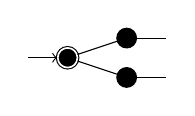
\begin{tikzpicture}[
    every node/.style={circle, draw, fill=black, inner sep=1pt, minimum size=2.5mm},
]
  \node [double] (a) at  (0.5, 0.25)  {}  edge    [<-]        (0,0.25);
  \node []       (b) at  (1.25,0   )  {}  edge    [-]         (a)
                                          edge    [-]         (1.75,0);
  \node []       (c) at  (1.25,0.5 )  {}  edge    [-]         (a)
                                          edge    [-]         (1.75,0.5);
\end{tikzpicture}

\vspace{1mm}

\[t+1\]

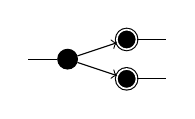
\begin{tikzpicture}[
    every node/.style={circle, draw, fill=black, inner sep=1pt, minimum size=2.5mm},
]
  \node []       (a) at  (0.5, 0.25)  {}  edge    [-]         (0,0.25);
  \node [double] (b) at  (1.25,0   )  {}  edge    [<-]        (a)
                                          edge    [-]         (1.75,0);
  \node [double] (c) at  (1.25,0.5 )  {}  edge    [<-]        (a)
                                          edge    [-]         (1.75,0.5);
\end{tikzpicture}


\vspace{6mm}


\[t\]

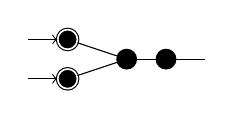
\begin{tikzpicture}[
    every node/.style={circle, draw, fill=black, inner sep=1pt, minimum size=2.5mm},
]
  \node [double]   (b) at  (0.5, 0   )  {}  edge    [<-]        (0,0);
  \node [double]   (c) at  (0.5, 0.5 )  {}  edge    [<-]        (0,0.5);
  \node []         (d) at  (1.25,0.25)  {}  edge    [-]         (b)
                                            edge    [-]         (c);
  \node []         (e) at  (1.75,0.25)  {}  edge    [-]         (d)
                                            edge    [-]         (2.25,0.25);
\end{tikzpicture}

\vspace{1mm}

\[t+1\]

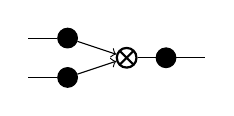
\begin{tikzpicture}[
    every node/.style={circle, draw, fill=black, inner sep=1pt, minimum size=2.5mm},
    cross/.style={path picture={
      \draw[black]
    (path picture bounding box.south east) -- (path picture bounding box.north west) (path picture bounding box.south west) -- (path picture bounding box.north east);
	}},
    crashed/.style={draw, cross, thick, fill=none},
]
  \node []         (b) at  (0.5, 0   )  {}  edge    [-]         (0,0);
  \node []         (c) at  (0.5, 0.5 )  {}  edge    [-]         (0,0.5);
  \node [crashed]  (d) at  (1.25,0.25)  {}  edge    [<-]        (b)
                                            edge    [<-]        (c);
  \node []         (e) at  (1.75,0.25)  {}  edge    [-]         (d)
                                            edge    [-]         (2.25,0.25);
\end{tikzpicture}

\vspace{1mm}

\[t+2\]

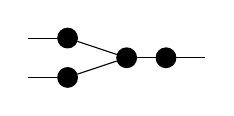
\begin{tikzpicture}[
    every node/.style={circle, draw, fill=black, inner sep=1pt, minimum size=2.5mm},
]
  \node []         (b) at  (0.5, 0   )  {}  edge    [-]         (0,0);
  \node []         (c) at  (0.5, 0.5 )  {}  edge    [-]         (0,0.5);
  \node []         (d) at  (1.25,0.25)  {}  edge    [-]         (b)
                                            edge    [-]         (c);
  \node []         (e) at  (1.75,0.25)  {}  edge    [-]         (d)
                                            edge    [-]         (2.25,0.25);
\end{tikzpicture}


\vfill

\end{minipage}%
%
\hfill%
\begin{minipage}{.75\textwidth}
\includegraphics[width=\textwidth]{raetsel/network}
\end{minipage}
